\documentclass[10pt,a4paper]{article}

\pdfinfo{
/Title (Implementation B)
/Subject (BDI learning)
/Author (Stephane Airiau)
/Keywords (coalition formation, cooperative game theory)
/Creator (LaTeX 2e)
/Producer ()}


\textheight 24.7cm
\textwidth 16cm
\headheight 0in
\headsep 0in
\oddsidemargin 0cm
\evensidemargin 0cm
\topmargin 0in


\usepackage[pdftex]{graphicx}
\usepackage{epstopdf}
\usepackage{amssymb,amsthm,amsfonts,mathrsfs}
\usepackage{subfigure}
\usepackage{pgf,tikz}
\usetikzlibrary{calc,arrows,shadows,fit,shapes,matrix,automata,positioning}
%\pagestyle{empty}


\usepackage{newcent}
\usepackage[T1]{fontenc}
\usepackage{amssymb,amsfonts,mathrsfs}
\usepackage[ruled,vlined]{algorithm2e}
%\usepackage{times}
%\usepackage[round]{natbib}

\begin{document}

{\bf Implementation B:} Regardless of whether we have seen world W
before, always use the average coverage of all previously seen worlds.

I agree, this will be monotonic. The average of coverage over all the
seen instances/worlds will provide some information about the quality
of the decision tree.  We can use that implementation for the paper.
What I have in mind is a bit more focused on the subspace that
contains the current new instance (already seen or not):

{\bf Implementation C:} Regardless of whether we have seen world W
before, always use the average coverage of all previously seen worlds
contained in the leaf node of the decision tree.

Let us say that for a plan with have the decision tree of
Figure~\ref{dt1}. And say we have a new instance $a \land b \land
\lnot c$. With the current decision tree, we see that it is currently
classified as a failure. 

I may or may not have seen the particular instance, and for now, the
decision tree provides an hypothesis.  What I want to know is how
reliable this hypothesis is. Using your idea of coverage, we can
consider the set $S$ of observed instances contained in the leaf node
$a \land \lnot c$ and compute the coverage offered by these instances
(i.e. we focus our attention only on the subspace satisfying $a \land
\lnot c$, we disregard its complement).

If the structure of the decision tree is correct (or if at least this
leaf node is correct), all the instances in $S$ lead to a similar
outcome. However, the way each instance is handled down the gptree may
be different. 

We should be able to guarantee monotonicity, but it will probably not
be so simple to be formal.  For example, the decision tree expands one
of the node (decision tree of Figure~\ref{dt2}, the node $a \land
\lnot c$ from Figure~\ref{dt1} is expanded using the attribute
$b$). We can still talk about the node $a \land \lnot c$ and even
after the split, the coverage will increase (though we will not care
about its value as only leaf nodes are of interest). If the change of
structure of the decision tree is larger, some nodes may cease to
exist, and may come back to existence after some changes in the
decision tree (and by then, the value of the coverage is larger).
This important changes of structures are very likely during the early
stages of learning, especially since we rebuild the tree from scratch
each time.

For sure, implementation C is more costly as each time the decision
tree changes, we need to check the coverage for each node (i.e., need
to go over each leaf node and compute the average). My intuition is
that if some subspace is found to work well, probably its coverage
will increase faster with implementation C than with B. 

\begin{figure}
\begin{center}
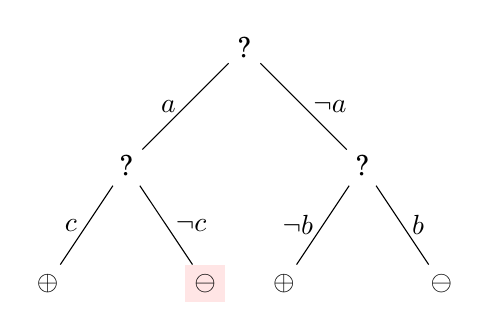
\begin{tikzpicture}[level 1/.style={sibling distance=30mm},
                    level 2/.style={sibling distance=20mm},
                    level 3/.style={sibling distance=15mm}
]

\node {?} 
child {node {?} 
    child {node {$\oplus$}  edge from parent node[left] {$c$}}
    child {node [fill=red!10] {$\ominus$}  
            edge from parent node[right] {$\lnot c$}
          }
       edge from parent node[left] {$a$} }
child {node{?}
    child {node {$\oplus$} edge from parent node[left] {$\lnot b$} }
    child {node {$\ominus$} edge from parent node[right] {$b$}}
edge from parent node[right] {$\lnot a$} };
 
\end{tikzpicture}
\end{center}
\caption{Decision tree for a plan}
\label{dt1}
\end{figure}

\begin{figure}
\begin{center}
\begin{tikzpicture}[level 1/.style={sibling distance=30mm},
                    level 2/.style={sibling distance=20mm},
                    level 3/.style={sibling distance=15mm}
]

\node {?} 
child {node {?} 
    child {node {$\oplus$}  edge from parent node[left] {$c$}}
    child {node {?}  
             child {node {$\oplus$}  edge from parent node[left] {$b$}}
             child {node {$\ominus$} edge from parent node[right] {$\lnot b$}}
            edge from parent node[right] {$\lnot c$}
          }
       edge from parent node[left] {$a$} }
child {node{?}
    child {node {$\oplus$} edge from parent node[left] {$\lnot b$} }
    child {node {$\ominus$} edge from parent node[right] {$b$}}
edge from parent node[right] {$\lnot a$} };
 
\end{tikzpicture}\end{center}
\caption{Decision tree for a plan}
\label{dt2}
\end{figure}

\textit{Dhirendra adds:} Ok, so this change would mean that we modify the probability update function of Section 5.2. The current definition is:
\begin{equation}
\label{eqn:coverage1} 
p'_n(W)= 0.5 + \left[  c_n(W) *  \left( p_n(W) - 0.5 \right)  \right]
\end{equation} 
where $c_n(W)$ is the average coverage of GPT node $n$ $\forall W$.

For Implementation C this would be changed to:
\begin{equation}
\label{eqn:coverage2} 
p'_n(W)= 0.5 + \left[  c_d(S) *  \left( p_n(W) - 0.5 \right)  \right]
\end{equation}
where $c_d(S)$ is the average coverage of DT node $d$ for subspace $S$ given $W \in S$.

This way as some subspace $S$ is found to work well, the biased probability $p'_n(W)$ will start to favour the subspace $S$ where $W \in S$ regardless of how $S$ is handled in the GPT hierarchy. This is a nice property. 

On the other hand it is hard to say how Implementation C will compare to Implementation B. C will be more focussed yes, but that could also be misleading since $S$ most likely will not be correctly defined (in the DT) in the early stages of the experiment.

\end{document}
